\section{Versuchsdurchführung}
\subsection{Versuchsaufbau}
Für den Versuch wurde die Anordung gemäß \autoref{fig:messaufbau} verwendet. Die Ladung des Zählrohrdrahtes löst am 
Widerstand einen Spannungsimpuls aus, der am Kondensator entkoppelt wird. Anschließend wird der Impuls 
verstärkt und am Zähler registriert oder an einem Oszillographen sichtbar gemacht. Die $\beta$-Strahlen 
Quelle wurde derart auf das Zählrohr gerichtet, dass die Zählrate $100$ imp/s nicht übersteigt, um 
Abweichungen aufgrund der vergleichsweise hohen Totzeit eines Geiger-Müller-Zählrohres zu vermeiden.
\begin{figure}
    \centering
    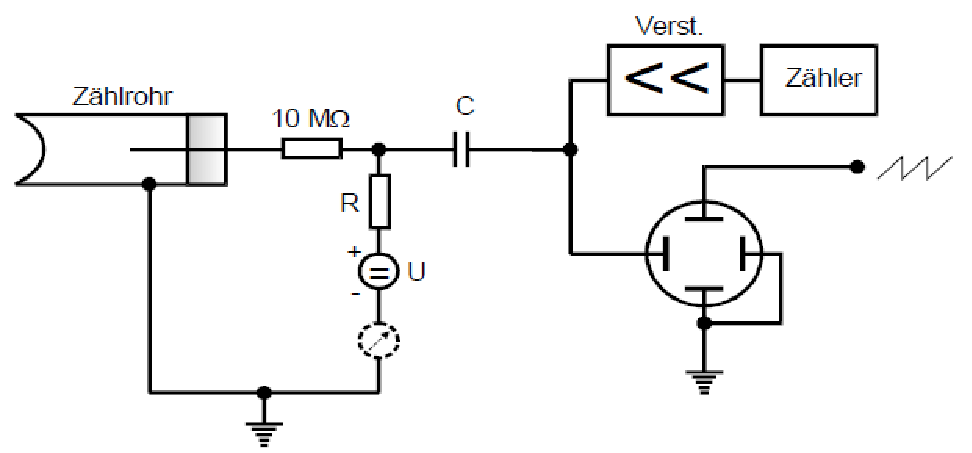
\includegraphics{Messaufbau.pdf}
    \caption{Pro einfallendem Teilchen ausgelöste Ladung Quelle: 1. TU-Dortmund, V703 Das Geiger-Müller-Zählrohr}
    \label{fig:messaufbau}
  \end{figure}
\subsection{Messung der Charakteristik}
Zur Messung der Charakteristik wurde die Spannung in Intervallen von $10 V$ erhöht, und die Zahl der Impulse 
pro 60 s gemessen. Diese Zeitspanne wurde gewählt, um zu gewährleisten, dass die Zahl der Impulse in der 
Größenordnung $N=10000$  liegt, damit der Messfehler $\Delta N=\sqrt{N}$ ca. 1\% oder geringer ist. 
Außerdem wurde die Zählrohrspannung in Abständen von $\Delta U=50 V$ gemessen.
\subsection{Messung der Totzeit}
\subsubsection{Oszillograph}
Die Totzeit kann bestimmt werden, indem von einem Oszillographen die Zeitspanne 
zwischen dem ursprünglichen Impuls und dem ersten nachfolgenden Impuls bei bekannter Ablenkgeschwindigkeit 
des Kathodenstrahls agelesen wird.
\subsubsection{Messung mithilfe der zwei-Quellen-Methode}
Um eine Totzeitkorrektur zur erhalten wurde die Impulsrate erhöht indem der Abstand zum Zählrohr verringert 
wurde. Anschließend wurde wie in \autoref{fig:zweiquellen} zunächst über $120s$  die Zählrate der ersten Quelle gemessen, anschließend wurde 
eine zweite Quelle hinzugefügt und zuletzt die erste Quelle entfernt und jeweils über die gleiche Zeitspanne 
gemessen.
\begin{figure}
    \centering
    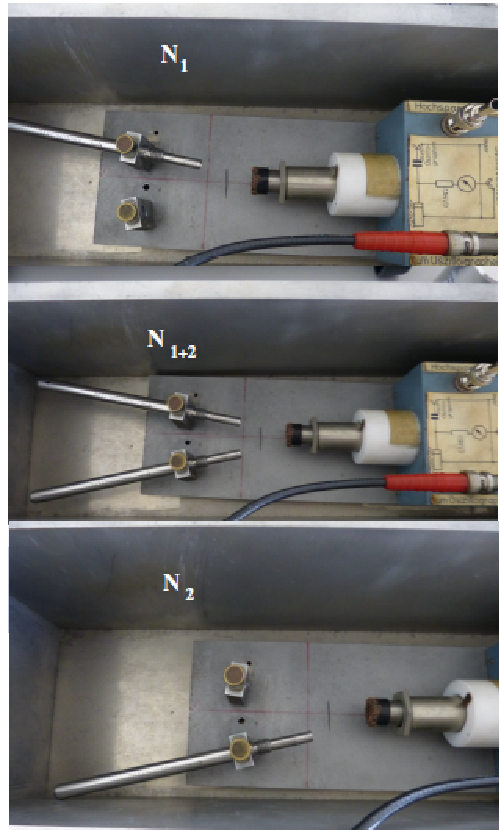
\includegraphics{Zweiquellenmethode.pdf}
    \caption{Pro einfallendem Teilchen ausgelöste Ladung. Quelle: 1. TU-Dortmund, V703 Das Geiger-Müller-Zählrohr
    \autoref{sec:literatur}}
    \label{fig:zweiquellen}
  \end{figure}
